\section{Methodologies and Experiments}
\begin{figure}
    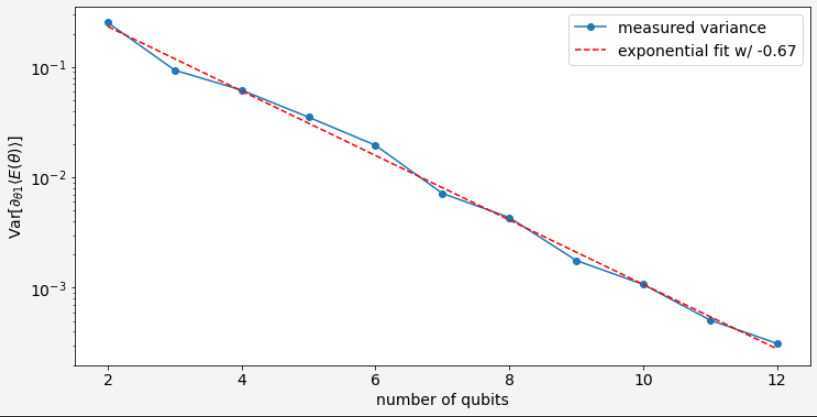
\includegraphics[width=\textwidth]{./ResearchDesign/Appendices/VarianceShrinking.png}
    \caption{
        An example of Barren Plateaus phenomenon occurs to a QNN model. 
        The variance of the gradient shrinking \textit{exponentially} with the number of qubits. 
        Barren Plateaus phenomenon prevents optimization algorithms to navigate the cost function landscape efficiently.
    }
    \label{Variance Shrinking demo}
\end{figure}

Cerezo et al. has pointed out that Barren Plateaus is cost function dependent \cite{cerezoCostFunctionDependent2021}, which implies that the only way to fully eliminate Barren Plateaus is to use a local cost function with a shallow circuit.
However, there are still other approaches to mitigate the phenomenon without using the local cost function.
The papers \cite{skolikLayerwiseLearningQuantum2021, liuParameterInitializationMethod2021} suggests that we can initiate the starting parameters away from plateaus to guarantee the trainability from the first steps.

First, we create a QNN model to reproduce the Barren Plateaus. 
We can use Qiskit to gain access to a wide range of ansatz, optimization algorithms, and most importantly the quantum emulator that capable of simulate up to 32 qubits.
The literature review also suggested that the two factors causing Barren Plateaus are the \textit{ansatz depth} and the \textit{randomised starting parameters}.
To reproduce the Barren Plateaus we force the QNN model to have one of the two factors, or both at the same time.
Then we calculate the variance of the gradient, and notice if the variance is shrinking \textit{exponentially} with the number of qubits (see Figure \ref{Variance Shrinking demo}).

\todo{I need to work on this section more, the methods sound trivial}

Then, we implement the three methods as discussed in the literature review.
The three methods will be applied to each QNN model (deep layered ansatz, randomised starting parameters, or both).
We will track the variances of the gradient for each QNN model and method.

After practising in a simulator, we experiment on the quantum hardware

From the data collected in experiment, we can conclude which method is the most suitable for different situation.

